\begin{frame}
Observation: Le modèle simple à deux niveaux avec peu de cables ne reproduit pas le problème. 

Nécessite d'étudier un problème un peu plus complexe:
%% \begin{figure}
%%   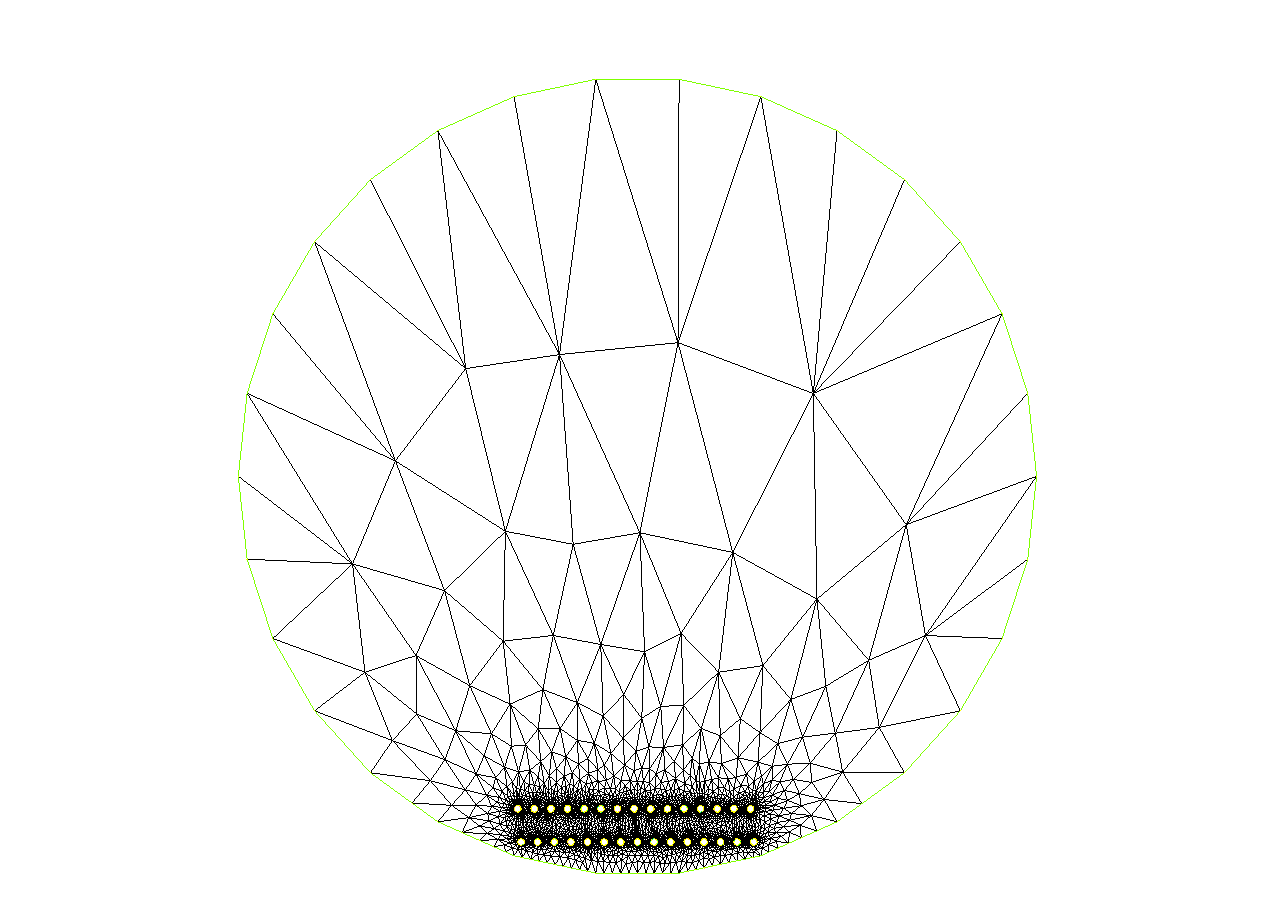
\includegraphics[scale=0.25]{../figs/bigcircle}
%%   \caption{Cas d'un blindage à deux niveaux}
%% \end{figure}
  \begin{figure}
    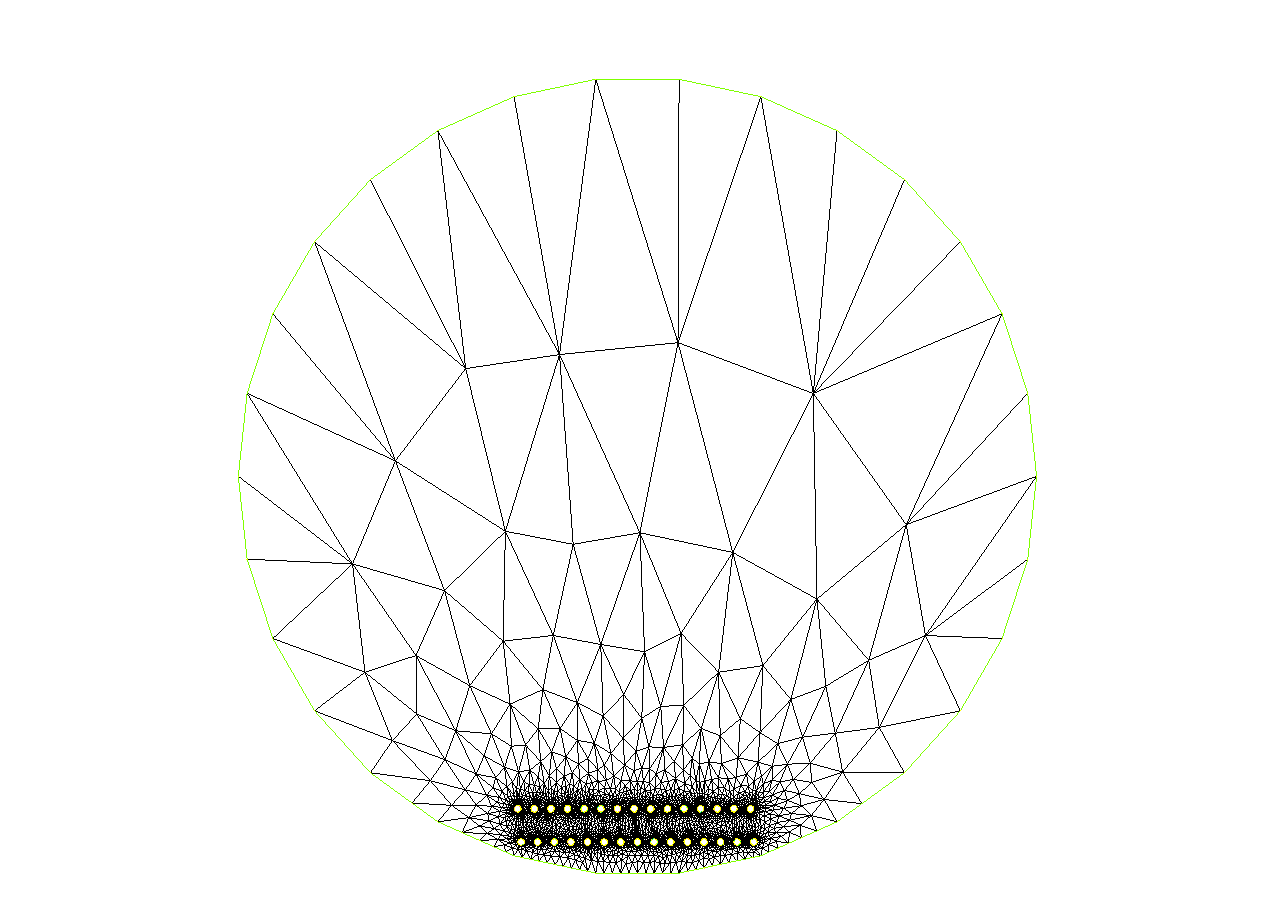
\includegraphics[scale=0.15]{../figs/bigcircle}  \hspace{1pt}
    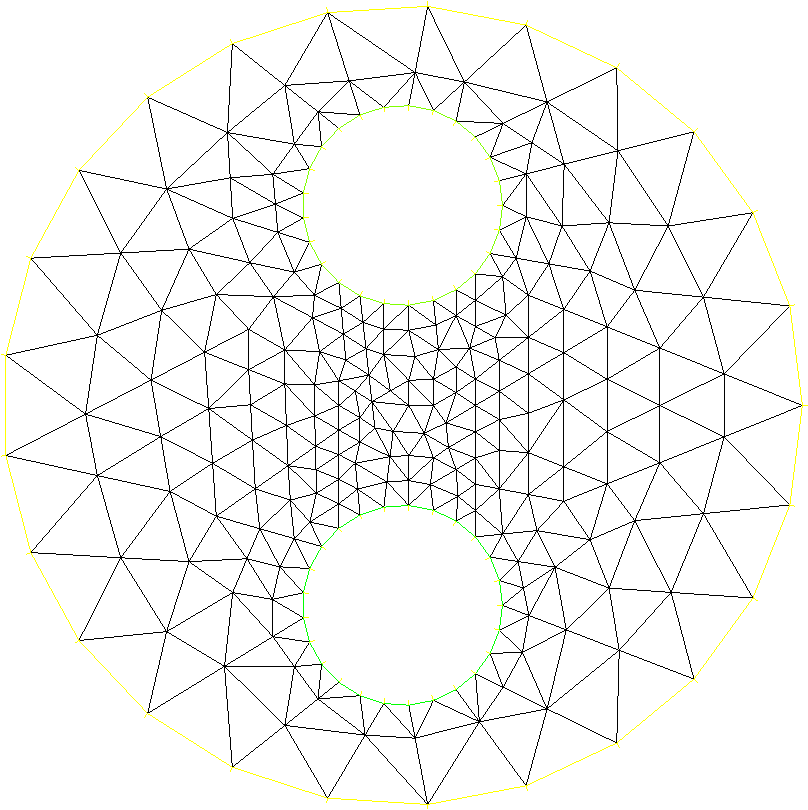
\includegraphics[scale=0.15]{../figs/Th1}  \hspace{1pt}
    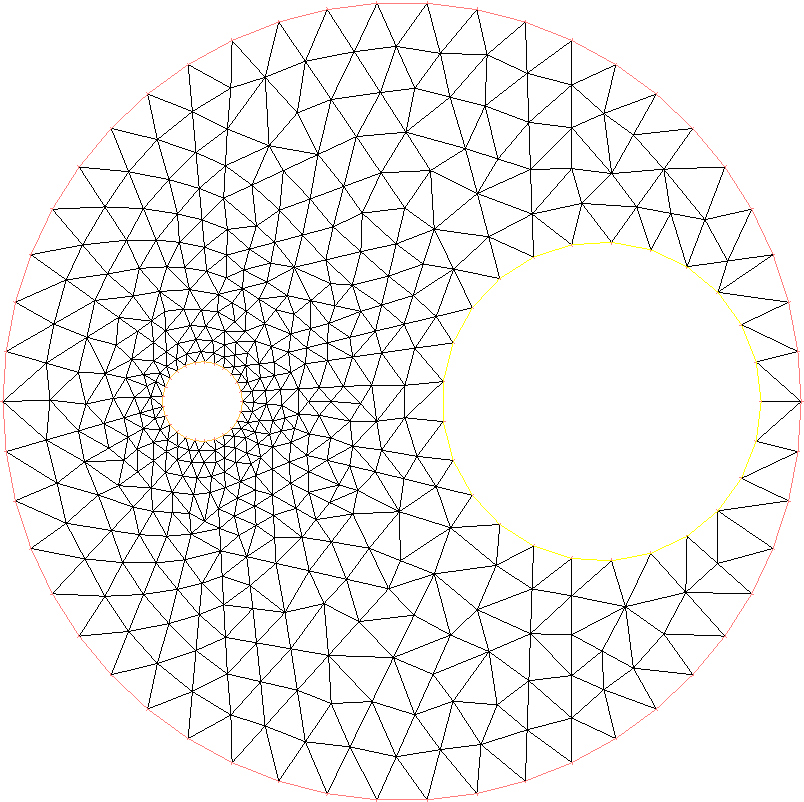
\includegraphics[scale=0.15]{../figs/Th0} \hspace{1pt}    
    \caption{Second blindage à deux niveaux}
  \end{figure}
\end{frame}

\begin{frame}
  \frametitle{Plan d'attaque}
  Procédure d'assemblage:
  \begin{itemize}
  \item Calculer les matrices $M$ du plus bas niveau vers le haut
    \begin{itemize}
    \item Définir la géométrie (FF++) 
    \item $M_{ij}$ nécessite d'introduire une certaine fonction $\psi_j$ localisée autour de $\partial w_j$ (pour obtenir une parfaite symétrie)
    \end{itemize}
  \item Procédures d'inversions de matrices denses ($M \to L$)
  \item Assembler $\delta$ sur le  niveau le plus haut puis la  matrice globale (Non achevé)
  \end{itemize}
\end{frame}

\begin{frame}
\frametitle{Exemple de solution}
TEST
%% \begin{figure}
%%   \includegraphics{../figs/exphi}
%%   \caption{Un exemple de solution du problème de Poisson}
%% \end{figure}
\end{frame}

\begin{frame}
  \frametitle{Observations}
  En pratique, difficultés rencontrées:
  \begin{itemize}
  \item Comprendre la théorie
  \item S'assurer que $M$ est bien symétrique:
    \begin{itemize}
    \item FreeFem++ : Automatisation des conditions aux bords multiples
    \item $\psi_j$ doit être parfaitement localisée: défauts de symétrie constatés dans le cas de simples projections.
    \end{itemize}
  \item Adapter le maillage.
  \end{itemize}
\end{frame}

\begin{frame}
\frametitle{Observations}

\begin{itemize}
  \item A tous les niveaux, $M,L$ ont les propriétés attendues
    \begin{itemize}
      \item Définies positive, $\kappa \simeq 15$
      \item Symétriques
    \end{itemize}
\end{itemize}


\begin{table}
\begin{tabular}{c|c|c|c}
 & Niv.1 & Niv. 2 & Niv.3\\
$M_{\text{ext}}$ & - & -& - \\
$L_{\text{ext}}$ & - & -& - \\
\end{tabular}
\caption{Temps de calculs}
\end{table}

\end{frame}
